\documentclass{article}

\usepackage{tikz}
\usetikzlibrary{arrows}

\begin{document}

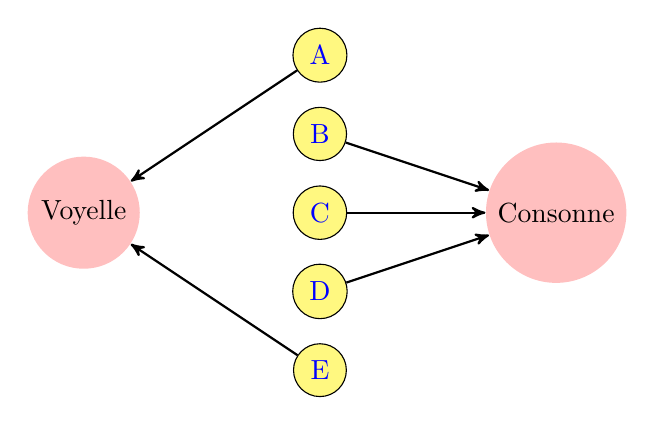
\begin{tikzpicture}
	\tikzstyle{lettre}=[circle,draw,fill=yellow!50,text=blue]
	\tikzstyle{type}=[circle,fill=red!25]
	\tikzstyle{fleche}=[->,>=stealth',thick]
	\node[lettre] (A) at (0,4){A};
	\node[lettre] (B) at (0,3){B};
	\node[lettre] (C) at (0,2){C};
	\node[lettre] (D) at (0,1){D};
	\node[lettre] (E) at (0,0){E};
	\node[type] (v) at (-3,2){Voyelle};  
	\node[type] (c) at (3,2){Consonne};
	\draw[fleche] (A) -- (v);
	\draw[fleche] (B) -- (c);
	\draw[fleche] (C) -- (c);
	\draw[fleche] (D) -- (c);
	\draw[fleche] (E) -- (v);
\end{tikzpicture}

\end{document}
